%!TEX program = xelatex
\documentclass[8pt, landscape, a4paper]{extarticle}

% --- 核心宏包 ---
\usepackage[UTF8, fontset=fandol]{ctex}
\usepackage[margin=0.8cm, top=1cm, bottom=1.3cm]{geometry}
\usepackage{multicol}
\usepackage{xcolor}
\usepackage{tcolorbox}
\usepackage{enumitem}
\usepackage{amsmath}
\usepackage{amssymb}
\usepackage{fontspec}
\usepackage{tikz}
\usetikzlibrary{arrows.meta}

% --- 去掉页码 ---
\pagestyle{empty}

% --- 颜色定义 (绿色主题) ---
\definecolor{headerblue}{RGB}{22, 160, 133}    % 主题绿
\definecolor{navcolor}{RGB}{211, 84, 0}        % 导航橙
\definecolor{intuitioncolor}{RGB}{41, 128, 185}% 直觉蓝
\definecolor{accentcolor}{RGB}{192, 57, 43}    % 强调红
\definecolor{section2}{RGB}{142, 68, 173}      % 紫色 (用于绘图)
\definecolor{dividergray}{RGB}{220, 220, 220}

% --- 全局设置 ---
\setlength{\parindent}{0pt}
\setlength{\columnsep}{0.4cm} 
\linespread{1.1} 

% --- 列表样式 ---
\setlist[itemize]{leftmargin=1.2em, nosep, itemsep=2pt, topsep=2pt, label=$\textcolor{headerblue}{\vcenter{\hbox{\tiny$\bullet$}}}$ }
\setlist[description]{leftmargin=0.2em, style=sameline, nosep, itemsep=2pt, font=\bfseries}

% --- Box 样式 ---
\newtcolorbox{mybox}[2][]{%
  colback=white,
  colframe=#2,
  coltitle=white,
  boxrule=1pt,             
  arc=2mm,                 
  left=4pt, right=4pt, top=3pt, bottom=3pt, 
  toptitle=3pt, bottomtitle=3pt, 
  fonttitle=\bfseries\sffamily\large,
  title={#1},
  after skip=5pt          
}

% --- 自定义命令 ---
\newcommand{\subt}[1]{{\vspace{2pt}\textbf{\large \textcolor{black}{#1}}}}

\newcommand{\boxdesc}[1]{%
    \textit{\small \textcolor{gray}{#1}}%
    \par\vspace{2pt}%
    {\color{dividergray}\hrule height 0.5pt}%
    \vspace{2pt}%
}

\newcommand{\sepline}{%
    \par \vspace{3pt}%
    {\color{dividergray}\hrule height 0.5pt}%
    \par \vspace{3pt}%
}

% 公式间距
\setlength{\abovedisplayskip}{3pt}
\setlength{\belowdisplayskip}{3pt}

\begin{document}

% --- 页眉 ---
\begin{center}
    {\Huge \textbf{\sffamily \textcolor{headerblue}{线性代数 Linear Algebra Cheat Sheet}}} \\
    \vspace{0.2cm}
    {\large \texttt{The Engine of Modern AI: From Matrix Transformations to SVD}}
\end{center}

% --- 开始四栏布局 ---
\begin{multicols*}{4}

% === 第一栏:空间与变换 ===

\begin{mybox}[��️ 场景导航 (Use Cases)]{navcolor}
    \boxdesc{遇到什么问题 $\to$ 用什么工具}
    \begin{itemize}[itemsep=1pt]
        \item \textbf{数据降维/压缩} $\to$ SVD / PCA
        \item \textbf{推荐系统/相似度} $\to$ 余弦相似度 (点积)
        \item \textbf{解线性方程组} $\to$ 逆矩阵 / 伪逆
        \item \textbf{图像旋转/缩放} $\to$ 线性变换矩阵
        \item \textbf{系统稳定性} $\to$ 特征值 (Eigenvalues)
        \item \textbf{概率分布变换} $\to$ 行列式 (Jacobian)
        \item \textbf{深度学习优化} $\to$ 梯度下降 / Hessian
        \item \textbf{数据投影/回归} $\to$ 最小二乘法 / QR分解
    \end{itemize}
\end{mybox}

\begin{mybox}[1. 空间与向量 (Spaces)]{headerblue}
    \boxdesc{万物皆向量,计算即变换}
    
    \subt{基本概念}
    \begin{itemize}[itemsep=1pt]
        \item \textbf{线性无关}: $\sum c_i v_i = 0 \iff \forall c_i=0$。
        \item \textbf{基 (Basis)}: 描述空间的最小坐标系。
        \item \textbf{秩 (Rank)}: 独立维度的数量。
        \item \textbf{张成 (Span)}: 所有线性组合构成的空间。
    \end{itemize}
    \sepline

    \subt{范数与度量 (Metric)}
    \begin{itemize}[itemsep=1pt]
        \item $\mathbf{L_1}$: $\sum |x_i|$ (Lasso, 稀疏解)
        \item $\mathbf{L_2}$: $\sqrt{\sum x_i^2}$ (欧氏距离)
        \item \textbf{点积}: $a \cdot b = |a||b|\cos\theta$ (投影)
        \item \textbf{正交}: $a \cdot b = 0 \iff a \perp b$
    \end{itemize}
\end{mybox}

\begin{mybox}[2. 矩阵与映射 (Matrices)]{headerblue}
    \boxdesc{矩阵不是数表,而是函数的描述}
    
    \subt{四大子空间 (The Big Four)}
    \begin{itemize}
        \item \textbf{列空间} $C(A)$: 值域 (Image)。
        \item \textbf{零空间} $N(A)$: 核 (Kernel),解 $Ax=0$。
        \item \textbf{行空间} $C(A^T)$ $\perp$ \textbf{零空间}。
    \end{itemize}
    \sepline
    
    \subt{秩-零化度定理 (Rank-Nullity)}
    $$ \text{dim}(N(A)) + \text{Rank}(A) = n \text{ (列数)} $$
    \textit{直觉:输入维度 = 损失的维度 + 保留的维度}

\end{mybox}

\columnbreak

% === 第二栏:核心分解 ===

\begin{mybox}[3. 特征值与特征向量 (Eigen)]{headerblue}
    \boxdesc{寻找变换中的“不动轴”}
    
    \textbf{定义}: $A$ 作用在向量 $x$ 上,仅伸缩不旋转。
    $$ Ax = \lambda x $$
    
    \sepline
    \subt{物理意义}
    \begin{itemize}
        \item \textbf{特征向量 ($x$)}: 矩阵的主轴、共振态。
        \item \textbf{特征值 ($\lambda$)}: 沿该轴伸缩的倍数。
        \item \textbf{迹 (Trace)}: $\sum \lambda_i = \text{tr}(A)$。
        \item \textbf{行列式 (Det)}: $\prod \lambda_i = \det(A)$ (体积)。
    \end{itemize}
    \sepline
    
    \subt{对角化 (Diagonalization)}
    若 $A$ 有 $n$ 个独立特征向量,则 $A = S \Lambda S^{-1}$。
    \textit{本质:换个基底,让变换变得纯粹(只伸缩)。}
\end{mybox}

\begin{mybox}[4. 奇异值分解 (SVD)]{accentcolor}
    \boxdesc{线性代数的“皇帝”公式}
    
    \textbf{任意}矩阵 $A$ ($m \times n$) 均可分解为:
    $$ A = U \Sigma V^T $$
    \begin{itemize}[itemsep=2pt]
        \item $U$: 左奇异向量 (正交),输出空间基。
        \item $\Sigma$: 奇异值 (对角),$\sigma_i \ge 0$,伸缩强度。
        \item $V^T$: 右奇异向量 (正交),输入空间基。
    \end{itemize}
    
    \sepline
    \subt{几何直觉}
    任何线性变换 = \textbf{旋转 ($V^T$)} $\to$ \textbf{拉伸 ($\Sigma$)} $\to$ \textbf{旋转 ($U$)}。
    
    \sepline
    \subt{应用:低秩近似 (PCA)}
    $A \approx \sum_{i=1}^{k} \sigma_i u_i v_i^T$
    \textit{保留前 $k$ 个最大的 $\sigma$,即保留了主成分。}
\end{mybox}

\begin{mybox}[5. 正定矩阵 (Positive Definite)]{headerblue}
    \boxdesc{矩阵里的“正数”}
    
    \textbf{定义}: $\forall x \neq 0, x^T A x > 0$。
    \begin{itemize}
        \item \textbf{性质}: 所有特征值 $\lambda_i > 0$。
        \item \textbf{几何}: 碗状函数 (凸函数),有全局最小值。
        \item \textbf{应用}: 优化问题 (Hessian)、协方差。
    \end{itemize}
\end{mybox}

\columnbreak

% === 第三栏:求解与应用 ===

\begin{mybox}[6. 线性方程组 (Solving $Ax=b$)]{headerblue}
    \boxdesc{从精确解到最优解}
    
    \subt{解的情况}
    \begin{itemize}
        \item \textbf{唯一解}: $A$ 可逆 ($\det \neq 0$)。
        \item \textbf{无解}: $b \notin C(A)$ (方程矛盾)。
        \item \textbf{无穷解}: $N(A)$ 非空 (有自由变量)。
    \end{itemize}
    \sepline
    
    \subt{矩阵分解求解 (LU)}
    $A = LU$ (下三角 $\times$ 上三角)。高斯消元的矩阵形式,计算机解方程的标准做法。
    \sepline
    
    \subt{数值稳定性}
    \textbf{条件数}: $\kappa(A) = \|A\| \|A^{-1}\| = \sigma_{\max}/\sigma_{\min}$。
    $\kappa$ 越大,矩阵越“病态”,解对误差越敏感。
    \sepline
    
    \subt{最小二乘法 (Least Squares)}
    当方程无解时,求误差最小的解:
    $$ A^T A \hat{x} = A^T b $$
    \textit{几何意义:将 $b$ 投影到 $A$ 的列空间上。}
\end{mybox}

\begin{mybox}[7. Python / Numpy 实战]{headerblue}
    \boxdesc{代码即数学}
    
    \subt{基础运算}
    \begin{itemize}
        \item 乘法: \texttt{A @ B} 或 \texttt{np.dot(A, B)}
        \item 逆/伪逆: \texttt{inv(A)} / \texttt{pinv(A)}
        \item \textbf{爱因斯坦求和}: \texttt{np.einsum('ij,jk->ik', A, B)}
    \end{itemize}
    \sepline
    
    \subt{SVD 与 PCA}
    \begin{itemize}
        \item \texttt{U, S, Vt = np.linalg.svd(A)}
        \item \texttt{S} 是奇异值数组,降维时取 \texttt{S[:k]}。
    \end{itemize}
    \sepline
    
    \subt{求解方程}
    \begin{itemize}
        \item 精确解: \texttt{x = np.linalg.solve(A, b)}
        \item 最小二乘: \texttt{x, \_, \_, \_ = np.linalg.lstsq(A, b)}
    \end{itemize}
    \sepline
    
    \subt{正交化 (QR)}
    \texttt{Q, R = np.linalg.qr(A)} (Gram-Schmidt)
\end{mybox}

\columnbreak

% === 第四栏:升维与直觉 ===

\begin{mybox}[8. 关键定理 (Theorems)]{headerblue}
    \boxdesc{支撑理论大厦的支柱}
    
    \subt{谱定理 (Spectral Thm)}
    任何\textbf{实对称矩阵} ($A=A^T$) 都可以被正交对角化。
    $$ A = Q \Lambda Q^T $$
    \textit{意义:对称矩阵极其完美,特征向量互相垂直。}
    \sepline
    
    \subt{Cholesky 分解}
    正定矩阵 $A = L L^T$。
    \textit{意义:矩阵的“开平方”,生成相关随机数。}
    \sepline
    
    \subt{Cayley-Hamilton}
    矩阵满足其自身的特征方程:$p(A) = 0$。
\end{mybox}

\vspace*{\fill}

\begin{mybox}[�� 核心直觉 (Intuition)]{intuitioncolor}
    \boxdesc{“矩阵是空间的折叠椅。”}
    
    % TikZ 矢量图:展示基变换/特征向量
    % 【关键修复】使用了 color=... 语法
    \begin{center}
    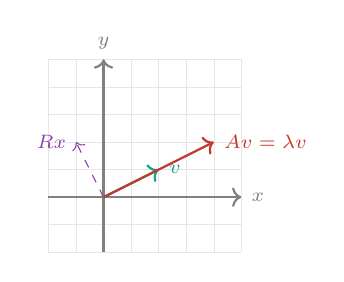
\begin{tikzpicture}[scale=0.7]
        \draw[step=0.5cm,gray!20,very thin] (-1,-1) grid (2.5,2.5);
        \draw[->,thick,gray] (-1,0) -- (2.5,0) node[right] {\scriptsize $x$};
        \draw[->,thick,gray] (0,-1) -- (0,2.5) node[above] {\scriptsize $y$};
        \draw[->,thick, color=headerblue] (0,0) -- (1,0.5) node[right] {\scriptsize $v$};
        \draw[->,thick, color=accentcolor] (0,0) -- (2,1) node[right] {\scriptsize $Av=\lambda v$};
        \draw[->,dashed, color=section2] (0,0) -- (-0.5, 1) node[left] {\scriptsize $Rx$};
    \end{tikzpicture}
    \end{center}

    \hspace{1em}线性代数不仅仅是解方程,它是描述\textbf{空间变换}的语言。
    \vspace{4pt}
    
    \subt{三大核心视角}
    \begin{itemize}[itemsep=4pt]
        \item \textbf{矩阵即变换}: 
        一个 $m \times n$ 矩阵是将 $n$ 维空间扭曲、旋转、投射到 $m$ 维空间的操作。行列式告诉我们体积是扩大了还是缩小了(det=0 意味着空间被拍扁了)。
        
        \item \textbf{特征值即主轴}: 
        在混乱的变换中,寻找那些“只伸缩不旋转”的特殊方向。它们构成了系统的“骨架”(如人脸识别中的特征脸)。
        
        \item \textbf{SVD 即数据压缩}: 
        任何复杂的数据矩阵,都可以拆解为:旋转 $\to$ 缩放 $\to$ 旋转。扔掉小的缩放系数,就做到了去噪和压缩。
    \end{itemize}
    
    \vspace{6pt}
    \centering\textit{\footnotesize 数据是新时代的石油,而线性代数是提炼石油的炼油厂。}
\end{mybox}

\end{multicols*}

\end{document}